\chapter{Background}
\label{background}

In this chapter, the fundamental concepts necessary to understand 
this thesis are explained.
First, the general concept of panic buying,
its consequences and what may lead to panic buying is explained 
(see section \ref{panicbuying}).
Then, the fundamental theory of graph systems are 
introducted and multiple attributes to describe graphs are defined 
(see section \ref{graphbasics}).
Furthermore, the concept of random graphs and multiple random 
graph algorithms are described.
Next, the concept of information diffusion
and multiple algorithms to model information diffusion are introduced
(see section \ref{informationdiffsection}).
Finally, different human-based variables that 
correlate with the power consumption are described
(see section \ref{powerloadsection},).


\section{Panic Buying as a Result from Social Media Influence}
\label{panicbuying}

Among consumer behaviors that have become increasingly concerning in modern times, 
one that stands out is the phenomenon of panic buying.
It occurs when there is an unusual surge in sales of 
specific goods due to extraordinary situations, such as natural disasters, 
pandemics, or the spread of misinformation among the general population.
Currently, this phenomeon has gained interest during the COVID-19 pandemic,
where the demand for disinfectants, soap and toilet paper increased significantly
\cite{covidpanicbuying}. Nonetheless, panic buying is not a new behavior.
But there are other historical examples for panic buying behavior.
These include the Spanish Flu
in 1918, where there was an increasing demand for medications 
\cite{honigsbaum2013regulating}. Another example is the Cuban Missile Crisis 
in 1962, where the sales of canned foods increased significantly \cite{george2004awaiting}, 
Lastly, during hurricane Irma in 2017, the affected population bought
significantly more fuel, bottled water 
and other essential goods in anticipation of the hurricane \cite{irmahurricane},
leading to shortages.

There are multiple possible reasons for panic buying behavior. These reasons 
are described in the work of \textit{Prentice et al.}
\cite{prentice2022antecedents}. They include:

\begin{itemize}
    \item Peer Pressure: The knowledge that other people fear shortages and 
    stock-outs leads to people being influenced by their peers' fears and thus leads
    to them fearing shortages themselves, thus forcing them to also buy excessively.
    \item Sense of Security: Given the uncertainty that the general population
    feels during a crisis, people want to secure their own future. This is also
    the case for when people anticipate shortages due to their peers' fears 
    and behaviors. Thus, they participate in panic buying to the secure their
    own stockpile.
    \item Media Influence: The stories of shortages on the media
    lead to a distorted view that there exists a shortage, thus increasing 
    the people's fears that a shortage exists or is drawing near and consequently
    leading them to participate in panic buying.
\end{itemize}

One cause of special interest for this thesis is the influence of 
media on the panic buying phenomenom. 
Multiple reasons for why social media influences consumer demand, 
specifically in the case of the COVID-19 pandemic,
are discussed in the work of \textit{Naeem} \cite{naeem2021social}.
In his work, he noticed that since people are spreading their 
own experiences on social media, the messages generated from their peers feel
more personal and lead to a stronger reaction by increasing the will to 
socially distance and to stockpile supplies. Additionally, people are generally
influenced more easily by their friends' posts and advices on social media.
Moreover, since friend circles became more 
internationalized through the global nature of social media networks,
events in other countries and its
possible consequences for one's own country can be analysed, thus
leading to a reaction. As an example,
shortage of a specific good in one country can lead to people in other countries
assuming that the shortage may happen in one's own country, thus leading to 
panic buying in one's own country. 
The next discovery was that people in positions of authority and with expertise,
such as politicians, organizations and experts, can use social media to increase 
the outreach of their messages, leading to people talking about their 
recommendations and policies.
Last, it was also proven that social media may increase rumor spreading,
thus leading to panic buying \cite{naeem2022understanding}.
In conclusion, social media can both amplify the messages and rumors that lead to 
panic buying and it can amplify the messages of governments and organizations 
that may inhibit the panic buying phenomenom.



\section{Graph as a Representation of Social Media Networks}
\label{graphbasics}
Graph models are a valuable approach for modeling real-world systems.
A graph is an abstract structure that represents a set of objects and the 
relationship between the objects. 
This Thesis primarily focuses on social media networks
\cite{socialgraphexample}. Nonetheless, graphs can 
also be applied to other real-world systems, such as economic systems 
\cite{economicsgraph} or power grids \cite{powergraphexample}.


Per definition, a graph $G(V, E)$ consists of a set of vertices (or nodes) $V$ and a 
set of edges $E$. Each edge connects two nodes $x, y \in V$ and is 
written as $e=(x, y)$. This means that for all $e\in E$, the 
condition  $e \subseteq\{ (x, y) \mid x, y \in V  \}$ 
is valid.

There are multiple different subtypes of graphs. A directional graph is a graph 
whose edges have a source node $a$ and target node $b$, thus representing
a direction from $a$ to $b$. If the edges do not fulfill this 
condition, i.e. if the edges do not show a direction, a graph is unidirectional.
In addition, a graph may have attributes, also called weights, 
associated to its edges. These graphs are called weighted graphs.

There are also multiple metrics that can be calculated in a graph
and that show its characteristics. Relevant metrics are 
explained below \cite{basicnetwork}.
\begin{itemize}
    \item The degree $c_v$ of a node $v \in V$ is the number of edges connected to the
    node $v$. 
    \item The degree distribution $P_k$ is the probability distribution 
    of the node degrees $k$ over all nodes $V$ in the graph $G$
    \item The average path length $l$ is the average number of steps between
    the shortest paths for all possible node combinations in a graph.
    \item The clustering coefficient $C$ describes how densely connected
    the vertices in the graph $G$ are. There are two different types of
    clustering coefficient. The global clustering
    coefficient is calculated as \\
    $C=\frac{(3 \cdot\text{number of triangles})}{(\text{number of connected triples})}$,
    where a connected triple means there are three nodes $a,b,c\in V$ with
    the edges $(a,b), (b,c) \in E$ (and where the edge $(a,c)$ may 
    possibly exist) and the number of triangles mean
    that the three vertices $a,b,c\in V$ that are fully connected to each other.
    The local clustering coefficient is calculated for a single node $i$
    and is defined as $C_i=\frac{\text{number of pairs of neighbors of }i 
    \text{ that are connected to each other}}
    {\text{number of pairs of neighbors of }i }$.
\end{itemize}

Furthermore, graphs that specifically model networks follow two special 
characteristics that may differ from other types of graphs.
First, network models are often scale-free networks.
Scale-free networks are networks that follow the power law distribution.
This law says that the degree distribution of a network
$P_k$ follows the power distribution.
This means that the probability that a node has a certain degree $k$ 
is proportional to the function $k^{-\gamma}$, where
$\gamma>1$.
On the other hand, most nodes are not directly
connected to one another in a small-world network.
Nonetheless, it is likely that they share the same neighbors or that their
neighbors share the same neighbors. 
Thus, most nodes can reach most other
nodes in the network by a small number of steps. For a network
to be considered a small-world network, its average path length $l$ 
needs to fullfil the condition $l\sim ln(n)$, where $n$ is the number
of nodes in the graph \cite{wattsmodel}.

One network that is of special interest in this thesis are social networks.
Social networks describe how humans are socially connected. 
These networks may for example model friendship, scientific co-authorship 
or online social media networks \cite{basicnetwork}. 
These kinds of networks can be modeled as graphs, where the nodes 
are the general population modeled in the system
and the edges model the relationship between the 
different people.
Social networks often share similar characteristics. The study of 
\textit{Mislove et al.} that focuses on online social media networks
shows, that social networks fulfill the small world characteristic,
have a high clustering coefficient and are scale-free networks
\cite{mislovesocialnetworkcharacteristics}. Thus, to accurately represent 
social networks, a graph should ideally fulfill all three characteristics.

\subsection{Random Graphs}
\label{randomgraphssection}
Graphs do not need to be based on real systems. They can also be generated. 
These randomly generated graphs are called random graphs \cite{randomgraphs}.
Typically, specific attributes in a random graph, such as the number of nodes 
or the number of edges, are predetermined, 
while other features are randomly generated using designated algorithms.

There are a number of algorithms used to generate random graphs.
The most commonly used algorithms are introduced in this section.

\subsubsection{Erdős–Rényi Model}

The oldest random graph algorithm is the 
Erdős–Rényi (ER) random graph. For this type of random model, the
number of nodes $n$ and the probability $p$ that an 
edge exists between two nodes are of fixed value \cite{basicnetwork}. 
To generate an ER random graph, the algorithm goes through 
every possible node combination $a, b$ and it creates an edge 
$(a, b)$ given the probability $p$. 
Thus, the number of edges $|E|$ is not fixed.

The characteristics besides the number of nodes and the
probability of the ER graph are generally not known.
Nonetheless, the average value of the other
characteristics to analyse the random graph algorithm can be calculated.
The graph characteristics of this type of random graph are shown in Table 
\ref{erdos-model}.
An important observation is that 
the average degree distribution $P_k$ follows the Poisson distribution
$P_\lambda (k) = \frac{\lambda^k}{k!}\, \mathrm{e}^{-\lambda}$. Thus,
ER graphs do not follow the power law distribution and are consequently
not scale-free. 

\begin{table}[ht!]
    \centering
    \begin{tabular}{|c | c |} 
     \hline
     Mean Number of Edges & 
     $\overline{|E|} = \binom{n}{2}p$  \\ 
     \hline
     Mean Degree & 
     $\overline{c} = (n-1)p$ \\ 
     \hline
     Degree Distribution & 
     $P_k = e^{-\overline{c}} \frac{\overline{c}^k}{k!}$ \\ 
     \hline
     Clustering Coefficient & 
     $C=\frac{\overline{c}}{n-1}=p$ \\ 
     \hline
     Average Path Length \cite{averagepath}& 
     $l = \frac{\ln{n} - \gamma}{\ln(\overline{c}))} + \frac{1}{2}, 
     \gamma=0.57722$ \\ 
     \hline
    \end{tabular}
    \caption{Mean characteristics of the ER random graph \cite{basicnetwork}}
    \label{erdos-model}
\end{table}

\subsubsection{Barabási–Albert Model}

Another well known random graph algorithm is the Barabási–Albert (BA) model 
\cite{barabasimodel}. 
This type of model uses the concept of preferential attachement.
To generate a graph based on this concept, first a small \glqq core\grqq{}
graph with $a$ nodes is created, where $a\ll n$ and $n$ is the final amount of nodes.
Then, $n-a$ nodes are sequentially added to the graph.
These nodes have a higher 
probability to connect to vertices that are already well-connected. 
Thus, the probability $p_i$ that a new node forms an edge with an
existing node $i$ depends on its degree $c_i$. This means that the
probability can be calculated as $p_i= \frac{c_i}{\sum_{k}c_k}$.
This concept of preferential attachement leads to the degree distribution
$P_k\sim k^{-3}$. Thus the BA graph 
fulfills the power law characteristic.
This can be seen in the graph characteristics of the random graph
in Table \ref{ba-model}. For this Table, $n$ is defined as the number
of nodes and $m$ as the number of edges that a node
will create when being added to the random graph.

\begin{table}[ht!]
    \centering
    \begin{tabular}{|c | c |} 
     \hline
     Degree & $c\geq m$ \\ 
     \hline
     Degree Distribution & 
     $P_k = \frac{2c_k(c_k+1)}{k(k+1)(k+2)}$ \\ 
     \hline
     Clustering Coefficient \cite{ba_cluster_coeff} & 
     $C=\frac{m}{8}\frac{ln(n)^2}{n}$ \\ 
     \hline
     Average Path Length \cite{averagepath}& 
     $l = \frac{\ln{n}- \ln{m/2} - 1 - \gamma}{\ln(\ln(n))+\ln{(m/2)}} + \frac{3}{2}, 
     \gamma=0.57722$ \\ 
     \hline
    \end{tabular}
    \caption{Mean characteristics of the BA random graph \cite{basicnetwork}}
    \label{ba-model}
\end{table}

\subsubsection{Watts–Strogatz Model}
The last random graph algorithm mentioned in this section 
is the Watts–Strogatz (WS) random graph \cite{wattsmodel}.
Contrary to BA random graphs, the focus of the WS graph is not to 
form graphs based on the power law, but to create graphs
that follow the small world characteristic more realistically.

The WS random graph model starts with a ring lattice graph, a graph 
with $n$ nodes where each node has the same degree $c$ and 
is connected to its $c$ nearest neighbors. Then, each edge $(a, b)$
may be rewired given the probability $p$, thus reconnecting the edge to  $(a, b')$
instead and creating a shortcut between the two non-neighboring nodes.
Furthermore, the new edge may only be created as long as it does not create
a loop $(a, a)$ and as long as the link $(a, b')$ does not already exist.
Another version of this algorithm does not rewire existing edges,
but creates new random edges as shortcuts given the probability $p$.
The second version creates a graph that can be considered more 
\glqq random\grqq{} as the graph generated in the first algorithm and is
thus favored over the former algorithm \cite{basicnetwork}.

The graph characteristics of the model can be seen
in Table \ref{ws-model}. Given the degree distribution $P_k$, it can be seen
that the distribution does not follow the power law since it is more similar
to the Poisson distribution than a power distribution. Thus, the WS model
is not scale-free.

\begin{table}[ht!]
    \centering
    \begin{tabular}{|c | c |} 
     \hline
     Degree Distribution & 
     $P_k = e^{-cp}\frac{(cp)^{k-c}}{(k-c)!}$ \\ 
     \hline
     Clustering Coefficient & 
     $C=\frac{3(c-2)}{4(c-1) + 8cp +4cp^2}$ \\ 
     \hline
     Average Path Length & $l = \frac{ln(ncp)}{c^2p}$ \\ 
     \hline
    \end{tabular}
    \caption{Mean characteristics of the WS random graph \cite{basicnetwork}}
    \label{ws-model}
\end{table}



\subsubsection{Comparison between the Random Graph Algorithms}
\label{comparison-random-graphs}
Analysing the average characteristics of all random graph algorithms introduced in
this chapter, it can be seen that they differ in their average graph characteristics.
The comparison of the different characteristics of all three models are shown 
in Table \ref{summary-graph-model}.
First, the ER model has comparatively low clustering coefficient compared to the 
other random graph models. Given a fixed average degree by defining 
the probability $p$ as $p=\frac{c}{n-1}$, the graph becomes less clustered
as the number of nodes of the graph increases. Both BA and WA model have higher clustering
coefficients compared to the ER model. Furthermore, for graphs with a 
high number of nodes $n$, the clustering coefficient of the BA model 
decreases. This is in contrast to the WA model, whose clustering coefficient 
does not depend on its graph size. Nonetheless, both models do not reach
the clustering coefficient metrics that can be seen in real social networks
 \cite{whatsappgraphmodels}.
Last, all three models fulfill the small-world characteristic $l\sim ln(n)$ 
and all models show similar values for the average path length
\cite{whatsappgraphmodels}.

\begin{table}[ht!]
    \centering
    \begin{tabular}{|c | c | c | c |} 
    \hline
     Characteristic & ER model & BA model & WA model \\
     \hline
     Scale-Free & \xmark & \cmark & \xmark \\ 
     \hline
     Clustering & Low & Middle & Middle \\ 
     \hline
     Small-World & \cmark & \cmark & \cmark \\ 
     \hline
    \end{tabular}
    \caption{Comparison of the three model types}
    \label{summary-graph-model}
\end{table}

\section{Information Propagation in Social Networks}
\label{informationdiffsection}
Since the creation of the internet, 
people are receiving increasing amounts of information.
This information is spread through social media.
Furthermore, both true and false information can spread through 
these channels.
Thus, the topic of information propagation over social media has become an 
important research field in the academic community.
The main way to analyse the spreading of information over a social network 
is by modeling the propagation process. The spread of information over 
a network is called information diffusion. 
The modeling of information diffusion can be divided into three components
\cite{reviewinformationdiffusion}: 

\begin{itemize}
    \item State: Entities in a system may be grouped together in a class which
    defines their behavior in the system. For example, 
    an entity can belong to the  \glqq Spreader \grqq{} class which 
    spreads the information
    to other entities in the system. An entity could also belong to a
    \glqq Susceptible \grqq{} class that did not receive the information yet, 
    but is able to receive it.
    \item Model: The model defines how the entities interact which each other
    given their states. A model is often represented by a graph with the entities
    as nodes and connections between the entities as edges 
    (see Section \ref{graphbasics}).
    \item Transition rates: The transition rates are the parameters used
    do define how the information is diffused in the model in a simulation. 
\end{itemize}

The first two components are independent of specific simulation scenarios,
unlike the third component. Thus the first two components should be further
analysed. Furthermore, there is a multitude of different ways 
to model information diffusion in social networks. Therefore, the most common
modeling methods will be further analysed in this chapter.

\subsubsection{Epidemiological Models}

Due to their similarity to the spread of infectious diseases, 
the spread of misinformation is often modeled in the same way as epidemiological models.
The simplest epidemiological model is the SI model, where entities in a system
can either belong to the state \glqq Susceptible\grqq{} ($S$) or 
\glqq Infected\grqq{} ($I$). Moreover, the number of total entities of a 
system can be calculated as $N=S+I$. The SI model is the basis for many
more specialised models where the states are more detailed to capture more 
aspects of real life behavior. A few models based on the SI model and their 
specific state are shown in Table \ref{SI-table}.

\begin{table}[ht!]
    \centering
    \begin{tabular}{|c | c |} 
     \hline
     Acronym & Classes  \\ 
     \hline
     SIR & Susceptible - Infected - Recovered  \\ 
     \hline
     SIS & Susceptible - Infected - Susceptible \\
     \hline
     SEI & Susceptible - Exposed - Infected \\
     \hline
     SIRS & Susceptible - Infected - Recovered - Susceptible \\
     \hline
     SEIR & Susceptible - Exposed - Infected - Recovered \\
     \hline
    \end{tabular}
    \caption{Example models based on the SI 
    model  \cite{reviewinformationdiffusion}}
    \label{SI-table}
\end{table}

Two models that shall be further analysed in this section are the SIR and SIS models. 
For the SIR model, it is assumed that at the beginning, all entities in the 
system are in the state $S$, thus susceptible to an infection. In the context of 
misinformation diffusion this means that an entity does not know about the
misinformation that is being spread and is neutral towards it. A susceptible
entity may become infected and thus may change its state to $S\to I$.
An infected entity knows and believes in the misinformation and may
spread the misinformation to other entities in the system. After being infected,
an entity may learn that the information is fake. Therefore, it recovers 
from being infected and changes its state to $I\to R$. An entity in a 
recovered state cannot be infected again by misinformation and thus is immune.
The SIS model differs from the SIR model in that the entity does not recover,
but it \glqq forgets\grqq{} about the fact that the information is fake 
and becomes susceptible to misinformation again.

The amount of entities belonging to each state may change 
after a time duration $\Delta t$. The equations to calculate the 
changes in number of entities in each state, and thus the progress 
of the information diffusion, can be seen in Table \ref{SI-table-equations}.

\begin{table}[ht!]
    \centering
    \begin{tabular}{|c | c |} 
     \hline
     SIR & SIS  \\ 
     \hline
     & \\
     $\begin{aligned}
          \frac{dS}{dt} &= -\beta I S \\
          \frac{dI}{dt} &= \beta I S - \gamma I \\
          \frac{dR}{dt} &= \gamma I  
        \end{aligned}$
      &
      $\begin{aligned}
          \frac{dS}{dt} &= -\beta I S + \gamma I\\
          \frac{dI}{dt} &= \beta I S - \gamma I
        \end{aligned}$
       \\ 
       & \\
     \hline
    \end{tabular}
    \caption{Model equations for SIR and SIS model \cite{sirequation}}
    \label{SI-table-equations}
\end{table}

$\beta$ and $\gamma$ are the transition rates parameters of the model, where 
$\beta$ is the transmission rate and $\gamma$ the 
recovery rate. Moreover, the equations in Table \ref{SI-table-equations}
are differential equations that are used to calculate the amount
of entities for each state in the system, not to calculate in which state
each entity in the system is in. Thus, the differential equations are 
only useful if a system-level view on the propagation is required.
If an entity-level view is necessary, i.e. if it is required to know which 
specific entities are in which state, then graph based diffusion models are needed.
There is no exact definition for an algorithm to calculate the state changes in the
graph model. Nonetheless, the probability that an entity changes
its state from susceptible to infected $S \to I$ generally increases depending on
how many neighbors are already infected. In its simplest form, a
propagation algorithm may be defined as in equation \ref{eqbasicpropagation} 
\cite{easypropagation}.

\begin{equation}
    I(a) = 1 (\sum\limits_{\substack{(b,a)\in E, \\ b \in V \cap I}}
    1(f^{\mathrm{rand}}\geq \beta)>0) 
    \label{eqbasicpropagation}
\end{equation}

In the equation, the infection status $I(a)$ of each node $a$ is defined 
by whether any neighboring node $b$ connected to $a$ is infected 
and fulfills the condition $f^{\mathrm{rand}}\geq \beta$.
The condition $f^{\mathrm{rand}}$ is the random probability generation function and $1$ 
is a function that equals one if the specific condition is fulfilled and 
zero otherwise. This means if any neighbor $b$ is infected and the 
condition $f^{rand}\geq \beta$ is fulfilled for $b$, then $a$ becomes infected. 
Afterwards, a node can recover given the probability $\gamma$.

Another method to model the information diffusion in an epidemiological model, 
specially the propagation of fake news and its debunking,
is described by \textit{Tambuscio et al.} \cite{sirsmodel}. In their work, they
define a modified type of SIS model where entities in the \glqq Infected\grqq{} 
are divided into two subgroups \glqq Believer\grqq{} and
\glqq Fact Checker\grqq{}.
The \glqq Believer\grqq{} subgroup believes in the fake news and spreads it 
to its neighbors.
The \glqq Fact Checker\grqq{} subgroup knows that the fake news is not 
true and only believes in the facts that are being spread. Furthermore, it
also spreads the factual information to its neighbors.

\begin{figure}[!ht]
    \center
    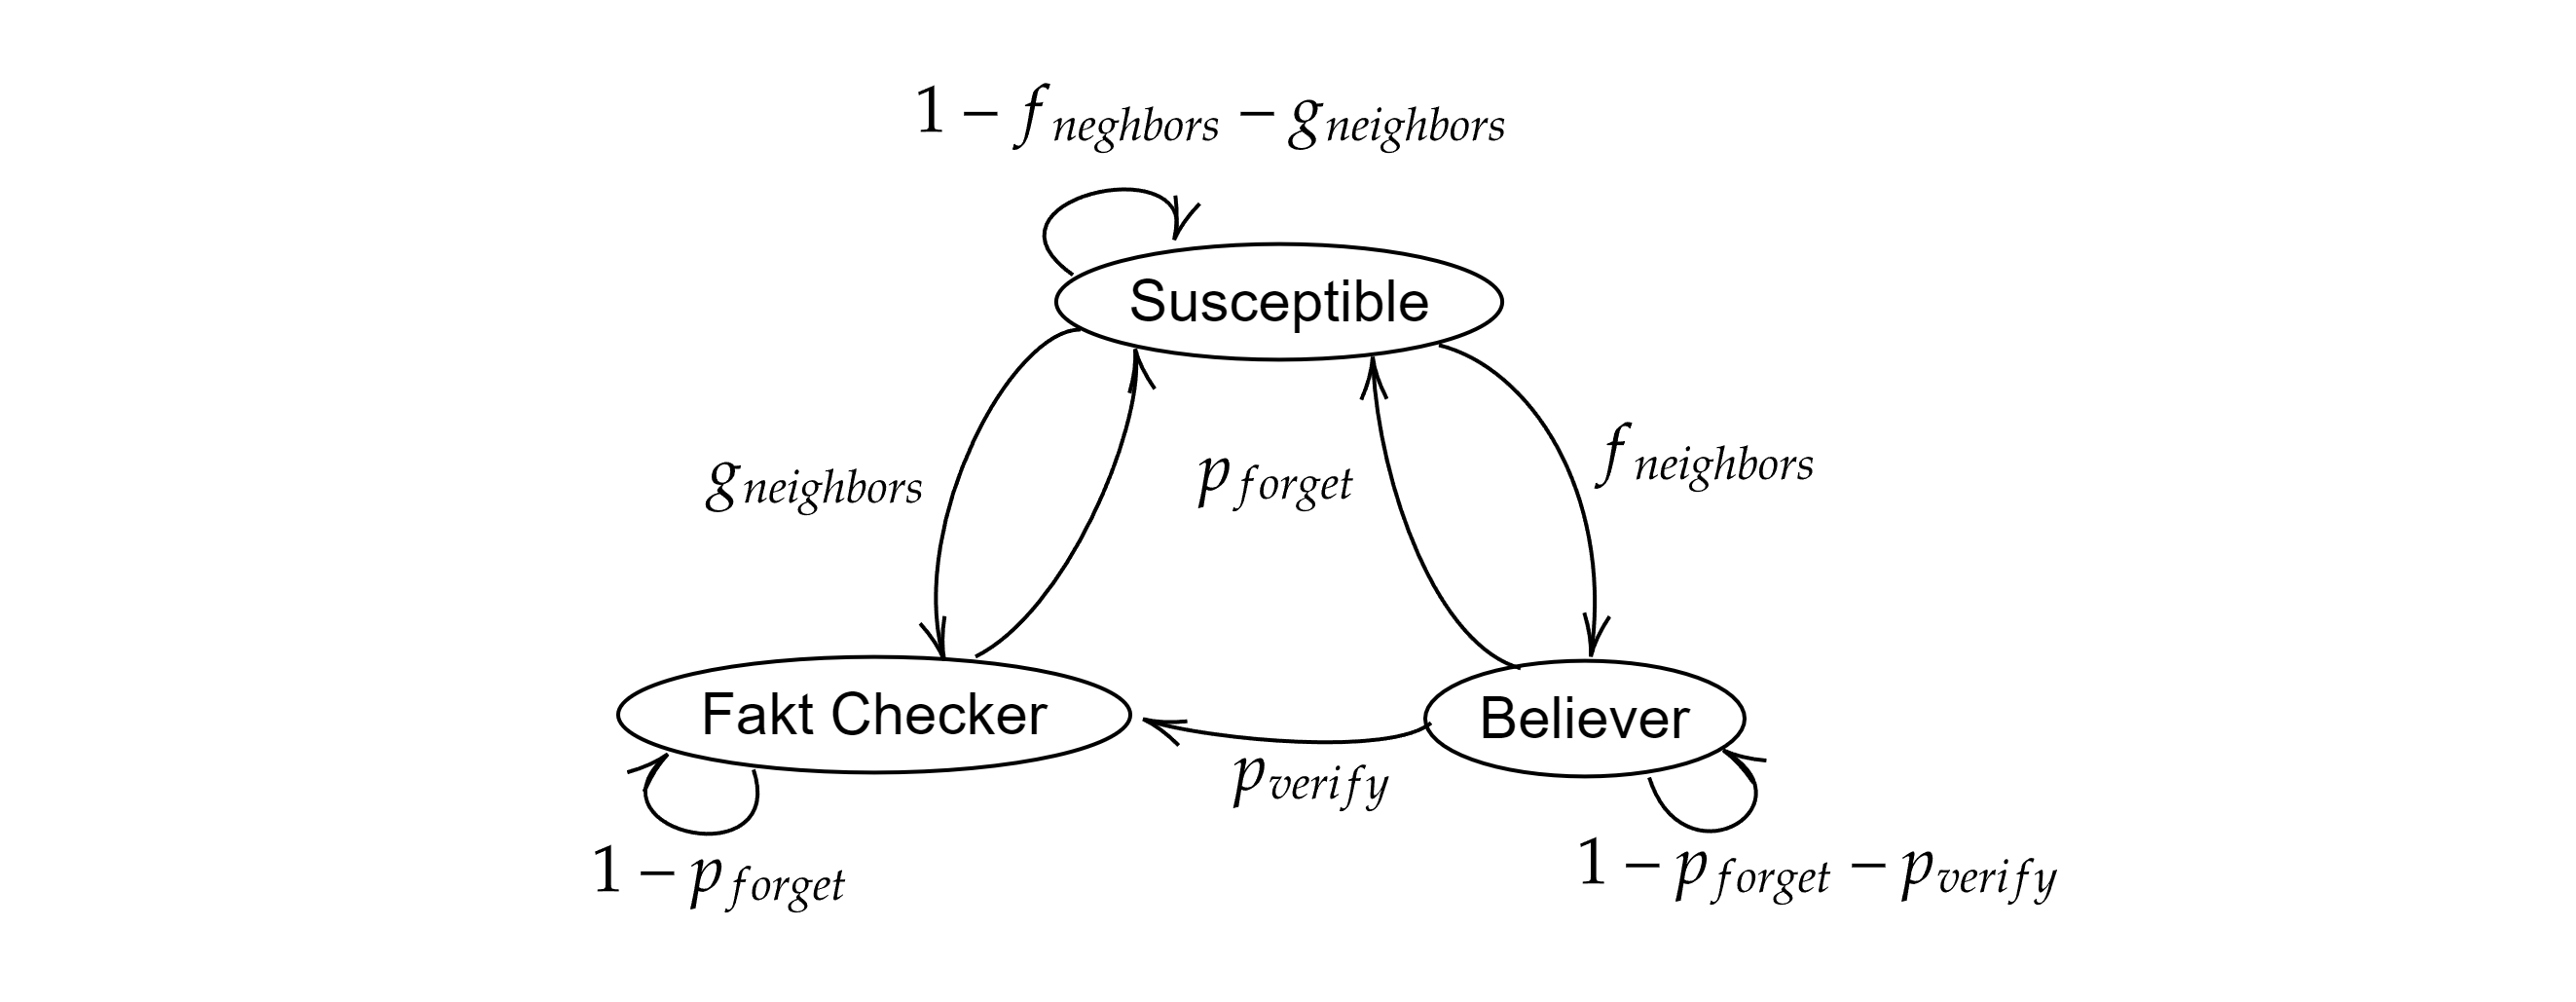
\includegraphics[scale=.15]{figs/Tambuscio.png}
    \caption{state chart for the model described
    in \textit{Tambuscio et al.} \cite{sirsmodel}}
    \label{originalmodelstatechart}
\end{figure}

\begin{table}[ht!]
    \centering
    \begin{tabular}{|c  c |} 
     \hline
     & \\
     $\begin{aligned}
          p_i^B(t+1) &= f_is_i^S(t) + (1-p_{forget}-p_{verify})s_i^B(t) \\
          p_i^F(t+1) &= g_is_i^S(t) + p_{verify}s_i^B(t)+(1-p_{forget})s_i^F(t) \\
          p_i^S(t+1) &= p_{forget}(s_i^B(t)+s_i^F(t)) + (1-f_i-g_i)s_i^S(t)
        \end{aligned}$
      &
      $\begin{aligned}
          f_i(t) &= \beta \frac{n_i^B(t)(1+\alpha)}{n_i^B(t)(1+\alpha)+n_i^F(t)(1-\alpha)} \\
          g_i(t) &= \beta \frac{n_i^F(t)(1-\alpha)}{n_i^B(t)(1+\alpha)+n_i^F(t)(1-\alpha)} \\
        \end{aligned}$
       \\ 
       & \\
     \hline
    \end{tabular}
    \caption{probability functions for the states described 
    in \textit{Tambuscio et al.} \cite{sirsmodel}}
    \label{SIS-table-equations}
\end{table}

In Figure \ref{originalmodelstatechart}, the states and the general probability
for transitions of the model are shown.
In Table \ref{SIS-table-equations}, the probability functions 
$p_i^B,  p_i^F,  p_i^S$ that a node $i$ will belong to each state  
\glqq Believer\grqq{}(B), \glqq Fact Checker\grqq{}(F) and 
\glqq Susceptible\grqq{}(S) at the iteration step $t+1$ are defined more clearly. 
These probability functions 
are dependent on the current state of the node $s_i=[s_i^B,  s_i^F,  s_i^S]$,
where $s_i^S$ is $1$ if the node $i$ has the state $S$ and else $0$.
Furthermore, the probability functions also depend on the constant system 
probabilities $p_{\mathrm{verify}}, p_{\mathrm{forget}}$. Last, the functions are also 
dependent on the propagation functions $f_i, g_i$, where $g_i$ describes 
the propagation of the fake news and $f_i$ the propagation of its debunking
for the node $i$. The two functions  $f_i, g_i$ are dependent on
the amount of neighbors $n_i^B, n_i^F$ that belong to the states
\glqq Believer\grqq{} or \glqq Fact Checker\grqq{} and the two 
system parameters $\beta$ and $\alpha$, where $\beta$ is the transmission rate
and $\alpha$ defines the credibility of the hoax. Thus, with this model it
is possible to model both the fake news spreading process and 
the fact-checking propagation process at the same time. 
Moreover, it is possible to consider the plausibility of the fake 
news in the propagation process.

\subsubsection{Information Cascade Models}

Another way to model information diffusion in graphs is by viewing it as a 
sequential information propagation process. This assumption is made in
information cascade models. In this type of model, any node $n$ infected in the
iteration step $i$ may infect its connected neighbor $a$ with a probability $P_n(a)$
\cite{reviewinformationdiffusion}. All nodes infected by node $n$
can then infect their neighboring node in the next iteration step $i+1$
and the node $n$ becomes inactive and does not infect any neighbors in any future
iterations.
The equation for the propagation step can be seen in equation 
\ref{eqbasicpropagationcascading}.
Information cascade models are mostly used for prediction and influence 
analysis purposes, and not to explain the collective behavior
of the system during the information diffusion process.

\begin{equation}
    I(a) = 1 (\sum\limits_{\substack{(b,a)\in E, \\ b \in V \cap I}}
    1(f^{rand}\geq P_n(a))>0) 
    \label{eqbasicpropagationcascading}
\end{equation}

There are several different subtypes of cascading models.
Some subtypes are described in \cite{diffusionbasics}. These are:

\begin{itemize}
    \item Independent Cascading Model: In this type of model, the 
    probability $P_n(a)=p$ ist constant for each node $a$ and neighbor $n$.
    Thus, the probability function does not depend on the history 
    of the system and its information diffusion status.
    \item Decreasing Cascading Model: In this type of model, the probability
    function to activate the node $a$ decreases with each attempts of its 
    neighbors. This means that if a neighbor $n$ unsuccessfully tries to infect
    $a$ at iteration step $i$, then the probability that the neighbor $m$
    can sucessfully infect $a$ at step $i+t$ is smaller, thus $P_n(a)>P_m(a)$.
\end{itemize}

\subsubsection{Threshold Models}
A different method to analyse the diffusion process in graphs is by viewing the
propagation step as a process where each entity needs to overcome a 
specific threshold $\theta$ to become infected. More specifically, 
a certain amount of neighbors need to be infected for node $a$ to become 
infected too. Furthermore, contrary to the cascade models, a node can always 
infect its neighbors as long as the conditions are fulfilled in the threshold 
model. The general equation for the threshold model can be seen in equation
\ref{eq:threshold}.

\begin{equation}
    I(a) = \sum\limits_{\substack{(b,a)\in E, \\ b \in V \cap I}}
    1 > \theta    
    \label{eq:threshold}
\end{equation}

Subtypes of this kind of diffusion model differ by the threshold parameter.
Some subtypes are described in \cite{diffusionbasics}. These are:

\begin{itemize}
    \item Majority Threshold Model: In this type of model, a node $a$ becomes
    infected if the majority of its neighbors are infected, thus 
    $\theta = \frac{1}{2}deg(a)$.
    \item Small Threshold Model: In this type of model, the threshold for that
    node $a$ becomes infected is very small. The advantage of this model is that 
    certain algorithms may be calculated faster with this type of model 
    \cite{diffusionbasics}.
    \item Unanimous Threshold Model: In this type of model, all neighbors 
    of a node $a$ need to be infected for $a$ to become infected, thus
    $\theta = deg(a)$.
\end{itemize}


\section{Variable Usages in Power Load Forecasting}
\label{powerloadsection}
% short introduction of power load forecasting 
% talk about 
A very significant task in modern power grid infrastructure management 
is to forecast
the future power demand, so that the power supply can be adjusted accordingly.
The power demand forecasting methods can be categorized in three types:
short-, medium and long-term power demand forecast. These differ in which
timespan they forecast the power demand. Most forecasting models are 
either statistical models or artifical intelligence-based models 
\cite{raza2015review}. But for these models to be able to predict the power 
demand, it is necessary to give them input data which correlate with the power 
usage. These kinds of variables that correlate with the power load 
can be classified as either endogenous or exogenous variables.
Exogenous variables can be considered as independent variables 
whose values determined outside of the system. 
Endogenous variables, on the other side, 
are variables that are dependent of other variables in the 
system.

In the context of power load prediction, the most commonly 
used endogenous variable is the historical power load data.
For the exogenous variables, there are multiple types of 
variables that are often considered as possible input data \cite{exogenousdata}
\cite{exogenousdata2}.
The first type of variables are environmental variables like temperature, 
rainfall, humidity or wind power. A different type of variables are time data
such as the specific weekday, if a day is a holiday and the time of the day.
One more type of variables are socio-economic variables such as the
population size and growth, the exchange rate, the income level,
the gross domestic product or the different types and amount 
of consumers like agricultural, industrial or household consumers.
Another type of variables are building and occupancy related variables such
as the household appliance usage,
the number of persons or the number of bedrooms in a household.

The relevance of each type of variables depend heavily on if the model is
a short-, middle- or long-term power load forecasting model. When shifting to more 
long-term predictions, the slower changing variables such as socio-economic
variables become more important than short-term variables such as weather data 
\cite{loadforecastingtimedependency2}\cite{loadforecastingtimedependency}.
The specific task definition is also relevant for the parameter selection.
Power load prediction models for residential buildings may benefit from 
building and occupancy related variables, but for a prediction model on a 
macroeconomic scale, socio-economic variables are more important.

Exogenous variables that are explicitly linked to human behaviour, 
such as social media usage, traffic information, satellite image data or 
internet usage, are not used often for power load forecasting. 
But these are the variables that would be affected the most in a change of 
human behavior. Thus, these variables should be analysed in more detail 
for this Thesis.

Social media data does not directly correlate with power demand, but it is
possible to extract information relevant for power demand prediction
from the content generated by it.
First, it is possible to analyse the spacial density of people by 
counting the amount of tweets tagged in a specific location of interest. 
In the work of \textit{Deng et al.},
it was shown that there is a significant
correlation between the amount of geotagged tweets
and the power consumption in a specific region \cite{twittergeoloccorr}.
As a possible explanation for this correlation, the paper assumes that 
an increased amount of human activity in a specific region leads a greater 
use of facilities such as heating or air conditioning in buildings or 
other types of power-consuming behavior.
For this reason, geotagged tweets were already used as input data for 
power load forecasting models 
\cite{twittergeolocforecasting} \cite{twittergeolocforecasting2}.
Second, it is also possible to analyse the content written in the 
social media posts. The content in social media posts can be 
analysed in two ways: 
It can either be analysed by searching for posts with a defined keyword or tag
or it can be analysed by using natural language processing techniques. 
In natural language processing the raw text content 
(and possibly its metadata and attachements) of a post is analysed
in some form to extract the desired information. Possible analysis
methods would be to classify if a post is related to some energy-consuming
behavior or to count the number of energy-relevant keywords in the text.
For example, a natural language processing model was trained to 
classify specifically energy-related tweets \cite{energybert}.
The other possibility is to query the social media instance 
to find all posts that contain the defined keyword or tag.
This method is usually simpler than using more sophisticated natural 
language processing techniques, but increases the amount of false positive 
posts that are not relevant for the specific task.
For power load prediction tasks, usually only the keyword search method is used.
In the work of \textit{LaLone et al.}, they show that the amount of energy
related tweets during hurricane Katrina correlated with the amount of 
power outages at the same time \cite{poweroutagetwitter}.
Another paper uses twitter data with both keyword search and 
tweets that were classified with natural language processing techniques to
to find power outage regions \cite{twitterpoweroutagelighttime}.
In addition, another paper used topic mining techniques to find
events on twitter posts that correlate with energy consumption 
\cite{twittertopicevent}.
Finally, a data type that can be considered as partially related to social 
network data, since it also shows the interest that greater parts of 
the population have for a specific topic, are search engine indices.
This was shown in the work of \textit{Wu et al.}, where it was proven that adding 
keyword search counts can improve power load forecasting accuracy 
\cite{googlepowerforecast}.

General internet traffic data also correlates with power usage.
In the study of \textit{Morleya et al.}, they conclude that 
electricity consumed by information and communication devices
may contribute to increased peak electricity demand 
\cite{internettrafficenergycorrelation}.
Therefore, internet traffic data can be used as input data for 
power demand forecasting models \cite{electricityinternetforecast}. 

Studies show that with the increased adoption of electric vehicles (EV), 
there is an increased interdependency between the electric and 
transportation infrastructure \cite{interdependnytrafficenergy}. 
Therefore, traffic data may correlate with power load 
in two ways:
First, with the traffic movement in general, it is possible to follow the
movement patterns of larger group. As an example, in the morning,
traffic intensity increases since larger part of the population needs
to go to their workplace. Subsequently, this population group
returns back to their residences after finishing their work in the afternoon.
Thus, there is also an increased traffic intensity in the afternoon.
This traffic movement can be analysed by measuring the 
incoming and outgoing traffic volume at the main roads of the 
region of interest. The usage of this variable in power load
forecasting models gained more interest during the COVID-19 pandemic, 
where drastically changing mobility and power consumption 
patterns meant that new model inputs were necessary to consider changing
behavior patterns in the general population 
\cite{covidtrafficpower} \cite{covidtrafficpower2}.
But this variable also correlates with the electricity consumption pattern
during normal times. One paper successfully showed that
using traffic data as an input for power load
forecasting models generally leads to more accurate predictions, even before
the COVID-19 pandemic \cite{causalmodeltrafficelectricity}.
Second, with the increasing EV usage in the future, 
the total power demand increases since these types of vehicles 
need to be charged often. Power load forecasting methods that consider this
issue often focus on charging stations \cite{evcharchingstations}
\cite{evcharchingstations2}, but changes in household power consumption 
and the general charging behavior of households
were also the objective of some studies. \textit{Gerossier et al.}
analysed in their study the different charging patterns in households
and found four different charging patters in which its members charged at 
a similar time and duration \cite{gerossier2019modeling}.
In addition, there are also studies that work on
power load prediction models for individual household
charging forecasts \cite{skala2023interval}. 
A notable study was done by \textit{Arias et al.} that also considered the traffic patterns
and analysed the differences in EV charging behaviors between
commercial and residential districts when forecasting the power demand
created by EV charging \cite{arias2016electric}.

The last variable that depends on human behavior mentioned in this section are
satellite images. These kind of images can be used to find a variety 
of enviromental factors that are of relevance for the amount of power demand.
Satellite images are mostly used to forecast power generation of 
renewable resources such as solar power \cite{solarprediction}.
But it can also be used to estimate household power consumption,
specially during nighttime. This is particularly of relevance for regions 
where the electricity data is unreliable, such as in developing contries
\cite{reviewnighttime}. There is a relation 
between nighttime light intensity and power consumption.
But this relation depends on the type of consumer, such as households, industry
or other types of consumers. Furthermore, the relation is not linear
\cite{nighttimepowerestimation}. 
A disadvantage of using nighttime images for power demand prediction is 
the inherent noise in the data. Non-household light sources such as 
streetlights and vehicles add noise to the image data \cite{reviewnighttime}.
Another usage of nighttime satellite image is for power outage detection.
If there is a power outage, the affected region will turn dark, which 
consequently can be detected in satellite images. Thus, satellite image data 
was successfully used in multiple power outage detection models
\cite{nightpoweroutage} \cite{twitterpoweroutagelighttime}.